% DTAG manuscript 2 -- Nature Human Behaviour-oriented ARTICLE DRAFT.
% Independent of dtag_main_new.tex; no changes to previous manuscript.
% This is a scientific redraft, not the publisher's typeset template.
% All numeric results derive from the completed 71-session calibrated
% human study, 960 native trajectories, 2880 fixed-set replays, and the
% investigator-reported item decomposition. Do not fabricate missing results.
% Original archived human data remain private.
%
% Editorial checklist before submission:
% - Verify institutional ethics review/exemption and approval reference;
%   recruitment dates, eligibility, compensation, screening and exclusions.
% - Verify sample characteristics, preregistration status and LLM interface
%   configuration (model version, prompts, validation and mapping error).
% - Freeze a code release and specify human-data access conditions.
% - Independently reproduce item-level exploratory tables from private export.
% - Confirm figure numbering and panel legibility at final print size.
%
\documentclass[11pt]{article}
\usepackage[T1]{fontenc}
\usepackage{lmodern}
\usepackage[margin=1in]{geometry}
\usepackage{amsmath,amssymb}
\usepackage{booktabs,tabularx,array}
\usepackage{graphicx}
\usepackage{microtype}
\usepackage{xcolor}
\usepackage[numbers,sort&compress]{natbib}
\usepackage[hidelinks]{hyperref}
\IfFileExists{lineno.sty}{\usepackage{lineno}}{}
\setlength{\parskip}{0.3em}
\setlength{\parindent}{1.25em}
\newcommand{\Ph}{\Phi}
\newcommand{\JS}{D_{\mathrm{JS}}}
\newcommand{\LSM}{\mathrm{LSM}}
\newcommand{\Iidx}{I_{\Ph}}
\newcommand{\Delt}{\Delta I_{\Ph}}
\newcommand{\pending}[1]{\textit{[To verify: #1]}}
\title{\bfseries Question selection shapes inferred political opinion and reveals resistance}
\author{Ishanu Chattopadhyay\\
\small Division of Biomedical Informatics, Department of Medicine,\\
\small University of Kentucky, Lexington, Kentucky, USA\\
\small Correspondence: \texttt{ishanu\_ch@uky.edu}}
\date{Working Article draft for \textit{Nature Human Behaviour}, 31 October 2026}
\begin{document}
\maketitle
\IfFileExists{lineno.sty}{\linenumbers}{}

\begin{abstract}
Surveys are used to infer political opinions from the answers people give, but those inferences also depend on which questions are asked. We tested whether adaptive selection of questions could systematically change an inferred opinion profile without specifying respondents' answers. A conditional model of the 2024 General Social Survey selected questions to shift a predictive left--right index. Directional movement occurred in 960 simulated trajectories and persisted in 2,880 fixed-question-set replays. In 71 completed human sessions, Left-directed questioning moved the index leftward in 20 of 21 participants; Right-directed questioning moved it rightward in 21 of 38. Among initially Left-leaning participants receiving Right-directed questions, 17 of 29 showed no net rightward movement. All 17 were identified by a four-answer nonmovement rule, with two additional participants flagged. These findings identify question-selection dependence and direction-specific resistance in \emph{model-inferred} opinion, rather than demonstrated changes in political beliefs.
\end{abstract}

\noindent\textbf{Keywords:} survey measurement; political attitudes; adaptive questioning; digital twins; belief systems; opinion structure; conditional inference.

\section*{Introduction}
Political attitudes are commonly inferred from responses to a finite battery of survey questions. The inference is often interpreted as a property of the respondent: an individual has a political position, and the survey reveals it. Yet a survey never observes the entire structure of a person's opinions. It observes a selected subset of statements, judgements and preferences, from which an analyst reconstructs what the person might say about other matters. The choice of questions can therefore matter even if the respondent answers each question without being instructed to adopt any particular position.

Work on belief-system constraint has long emphasized the incomplete and heterogeneous interdependence of mass political attitudes \citep{converse1964,zaller1992,baldassarri2008}. Survey research has also established that question context, wording and the process of formulating a response can influence what is reported \citep{schumanPresser1981,schwarz1999,tourangeau2000}. These literatures raise two distinguishable possibilities. The questions themselves may influence what people think or say; alternatively, different selections of answers may lead a measurement model to infer different positions even when the respondent's underlying beliefs do not change. The second mechanism is consequential for contemporary adaptive surveys and conversational systems, where an algorithm determines which evidence about a person becomes available.

We examine the latter mechanism through \emph{Digital Twin Anchored Generation} (DTAG), a system that uses a learned model of conditional survey responses to choose which question to ask next. The model represents a respondent by the predicted distributions of answers to unasked questions. Two reference profiles define a left--right coordinate within that predictive geometry. DTAG selects each question to maximize expected displacement of that coordinate in a specified direction; it does not select or prescribe the answer.

Our experiments separate model-generated responses from real participant responses. First, a controlled simulation begins from six stated General Social Survey (GSS) personas and draws every subsequent answer from a large science model (LSM) fitted to GSS 2024. A second experiment uses the same directional selection logic but substitutes answers supplied by recruited participants, interpreted through a natural-language interface. This distinction allows us to ask not only whether a question-selection policy can move its own inferred index under model-generated answers, but whether directional behavior and nonresponse are observed when humans provide the answers.

The central behavioral finding is an asymmetry: observed Left-directed movement was common, whereas Right-directed movement was substantially less frequent among those initially located nearer the Left reference pole. We use \emph{directional response phenotype} to describe this observed trajectory in a conditional model, and \emph{resistance} to describe the failure of a specified policy to achieve positive displacement in its intended direction. Neither term presupposes a fixed psychological type or a change in underlying belief. We further examine which question topics accompany directional displacement, and whether the early trajectory contains information about its eventual direction.

\section*{Results}

\subsection*{A person's inferred position depends on the observed answers}
We used the conditional response structure of a GSS 2024 LSM to form a predictive phenotype: for each unasked item, the model estimates the distribution of answers given the responses already observed. Distances between these model-predicted conditional profiles define an opinion geometry. We represented position by a scalar index relative to two reference states built from opposing answers on 27 GSS variables. The index equals $-1$ at the Left reference pole and $+1$ at the Right reference pole (Methods).

Consider a participant with an initial observed answer set $s_0$. After an additional answer is recorded, the model conditions on the enlarged set and recomputes predictions about unanswered items. The change in index, $\Delt(t)=\Iidx(s_t)-\Iidx(s_0)$, describes \emph{movement of the inferred phenotype}. It does not require the person to have changed an already-held opinion. The measurement is contingent on both the respondent's answers and the questions chosen to elicit them.

A Left-directed policy selects the next question expected to decrease this index; a Right-directed policy selects the question expected to increase it. Neutral and Random policies provide descriptive comparators. The selector always operates on the LSM conditional model. A language model is not used to generate answers in the native simulation, nor does it supply human participants' answers (Methods).

\subsection*{Model-generated respondents exhibit systematic directional displacement}
We initialized six stated GSS personas and simulated 40 independently sampled 20-question trajectories for each of four selection policies. This produced 960 trajectories and 19,200 LSM-generated answers. No item used to define the 27-variable reference poles was eligible for question selection. Across the six initial personas, Left- and Right-directed selection shifted the conditional index in the prescribed directions (Fig.~\ref{fig:nhb-native}). Neutral and Random policies provided comparisons.

\begin{figure}[!t]
\centering
\IfFileExists{Figures/External/dtag-fig1.pdf}{%
  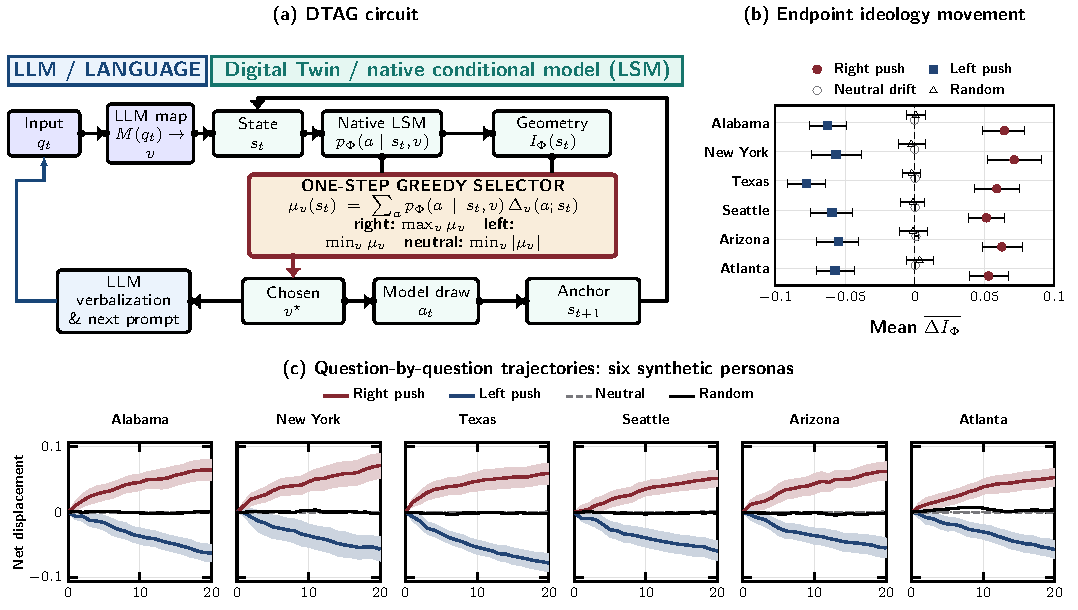
\includegraphics[width=.96\linewidth]{Figures/External/dtag-fig1.pdf}%
}{\fbox{\parbox{.89\linewidth}{Insert the already-committed DTAG native architecture and trajectory figure (\texttt{Figures/External/dtag-fig1.pdf}).}}}
\caption{\textbf{Adaptive question selection and native GSS simulations.}
The existing DTAG source figure combines (a) the conditional-model/question-selection architecture, (b) simulated mean endpoint displacements across six specified personas, and (c) 20-question mean trajectories under Left, Right, Neutral and Random policies. All simulated responses are sampled directly from the LSM conditionals, not generated by an LLM. Pole-defining questions are excluded. Confidence intervals are participant-persona simulation bootstrap intervals as specified in the original analysis.}
\label{fig:nhb-native}
\end{figure}

We then tested whether directionality required the continuous adaptive update or the exact ordering of the selected questions. For each of 18 persona--policy combinations (six personas crossed with Left, Right and Neutral), we froze a 20-item set from one adaptive replicate. Each set was replayed in its original, reversed and two shuffled orders using 40 fresh LSM response sequences per order, for 2,880 replays. The original and reversed Right-derived sets yielded mean displacements $+0.0381$ and $+0.0377$, respectively; the Left-derived sets yielded $-0.0399$ and $-0.0410$. Direction was retained under the tested shuffles as well. All 54 pointwise bootstrap intervals for paired between-order mean contrasts included zero (Extended Data Fig.~\ref{fig:nhb-order}). Thus, in these simulations, the selected \emph{question identities} retained directional information even without ongoing reoptimization.

\subsection*{Humans show asymmetric directional responses}
The prospective human study comprised 71 completed, six-question-calibrated Prolific sessions: Left ($n=21$), Right ($n=38$), Neutral ($n=7$) and Random ($n=5$). Each included 20 adaptive questions and five interleaved attention checks. Whereas model-generated experiments sampled responses from fitted conditional distributions, human participants supplied their own natural-language answers. A language-model interface mapped the answers into accepted native survey-variable observations, allowing the LSM to update its predictive state.

The observed Left-push mean endpoint displacement was $-0.0989$ (95\% participant-bootstrap interval $[-0.1200,-0.0741]$); the Right-push mean was $+0.0225$ ($[+0.0006,+0.0452]$). Neutral and Random mean changes were $-0.0054$ and $-0.0045$, respectively. Movement was leftward in 20 of 21 Left-push sessions (95.2\%) and rightward in 21 of 38 Right-push sessions (55.3\%; Fig.~\ref{fig:nhb-human}).

\begin{figure}[!t]
\centering
\IfFileExists{Figures/External/dtag-fig3.pdf}{%
  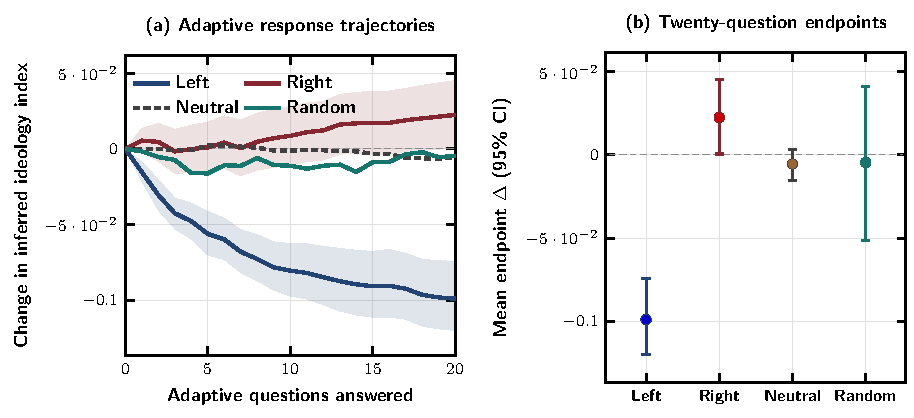
\includegraphics[width=.86\linewidth]{Figures/External/dtag-fig3.pdf}%
}{\fbox{\parbox{.85\linewidth}{Insert the committed four-panel, 71-person human-study figure (\texttt{Figures/External/dtag-fig3.pdf}).}}}
\caption{\textbf{Human responses to directionally selected questions.}
(a) Mean change in the LSM-inferred index after each of 20 questions; colored shaded bands show 95\% participant-bootstrap intervals for Left and Right policies. (b) Mean endpoint displacements for all four policies. (c) Directional movement stratified by baseline inferred index: initially Left/Left push, 16/17; initially Right/Left push, 4/4; initially Left/Right push, 12/29; initially Right/Right push, 9/9. (d) Among initially Left-leaning Right-push participants, a four-question early-nonmovement flag versus the full 20-question outcome: true positive 17, false positive 2, false negative 0, true negative 10. This is the original 71-session figure; no participant-level records are displayed.}
\label{fig:nhb-human}
\end{figure}

Baseline inferred position distinguished Right-push trajectories. Of 29 Right-push participants whose initial index was negative, 12 moved rightward (41.4\%). All nine Right-push participants with a positive initial index moved rightward (100\%). Left-directed movement occurred in 16 of 17 initially Left-leaning participants (94.1\%) and in all four initially Right-leaning participants (100\%). The difference between Right-directed responses in the two baseline groups is substantial as a descriptive pattern. In particular, the poor pooled Right-push response was concentrated among initially Left-leaning participants.

\subsection*{Early nonmovement identifies subsequent directional resistance}
We operationally defined Right-push endpoint resistance as $\Delt(20)\leq0$. Among the 29 initially Left-leaning participants assigned Right push, 17 met this definition after 20 questions. We examined a simple early flag: no positive baseline-relative displacement after the first four adaptive answers, $\Delt(4)\leq0$. This criterion flagged all 17 eventual endpoint nonresponders, as well as two participants who ultimately moved rightward. Its observed sensitivity was 17/17, precision 17/19 (89.5\%), specificity 10/12 (83.3\%) and accuracy 27/29 (93.1\%).

The early trajectory therefore differentiated outcomes in a specific directional subgroup. In the original archived population, applying this four-question flag removes 19 of 38 Right-push sessions: 17 eventual nonresponders and two eventual responders. The remaining Right-push trajectory comprises ten initially Left-leaning participants without the flag and nine initially Right-leaning participants. Extended Data Fig.~\ref{fig:nhb-unflagged} shows this Q4-conditioned trajectory beside the unchanged Left, Neutral and Random trajectories.

\subsection*{Cultural and civil-liberties questions accompany much of the leftward movement}
To begin explaining the asymmetry, we decomposed each observed 20-question trajectory into stepwise index increments and associated each increment with the selected GSS target question. This decomposition is exact at the question level: the sum of increments equals the baseline-to-endpoint change. Where a response maps to several survey variables, the increment belongs to the \emph{joint update}, not uniquely to each mapped variable (Methods).

For Left-push participants, questions concerning religion, sexual morality and civil liberties were prominent among those associated with positive leftward increments. The question coded \texttt{colath}---whether a person opposed to religion should be allowed to teach at a college---had the largest aggregate positive gain in both baseline groups: $0.09768$ across four selections among initially Right-leaning participants and $0.38915$ across 17 selections among initially Left-leaning participants. Positive gain per selection was similar in these groups ($0.0244$ and $0.0229$, respectively). Other prominent items among initially Right-leaning Left-push sessions addressed religion's influence (\texttt{religinf}), premarital sex (\texttt{premarsx}), assisted dying or suicide under terminal illness (\texttt{suicide1}), abortion when the woman's health is at risk (\texttt{abhlth}), and same-sex relations (\texttt{homosex}). These counts are \emph{question selections}, not counts of distinct participants.

We examined a predeclared category of spending and government-program questions as an exploratory test of the interpretation that symbolic conservatism can coexist with operationally liberal policy preferences \citep{ellisStimson2012}. Initially Right-leaning Left-push participants received spending/program questions more often than initially Left-leaning Left-push participants (mean shares 13.75\% versus 7.35\%; exact two-sided label-permutation $P=0.0894$). But the fraction of each person's total positive leftward increment magnitude associated with spending/program questions was almost identical (8.06\% versus 7.36\%; $P=0.8932$; 5,985 exact label permutations for each comparison). Spending/program selection therefore did not account for a greater share of positive leftward movement in the initially Right-leaning group. Instead, the question-level pattern points descriptively to cultural, religious and civil-liberties associations in the conditional opinion geometry.

\section*{Discussion}
The results expose a dependency that is easy to overlook in model-based political measurement: an inferred position can be a function of both the person's responses and the policy that selects which responses to observe. The LSM does not need to change a reported answer to change its inferred position. The same principle is relevant to adaptive questionnaires, automated interviews and any profiling system that builds a representation of a person from selectively acquired evidence. An audit confined to whether an answer was transcribed correctly would not characterize the effect of selecting that particular question rather than another.

The human study contributes more than a test of an optimization routine on its own simulated outputs. With participant-supplied responses, the conditional index shows substantial leftward displacement under Left-directed selection and a pronounced baseline-dependent asymmetry under Right-directed selection. These observations motivate a picture of \emph{directionally accessible} and \emph{directionally resistant} response phenotypes: the model can update toward one reference profile as particular observed answers arrive, yet another requested direction may not be attained over the same question budget. A resistant trajectory is scientifically informative even when the desired shift does not occur.

What makes movement possible? A first mechanism is \emph{selective revelation}. Real respondents may hold heterogeneous positions across cultural, political and institutional questions; an adaptive policy can elicit those observations that substantially change the model's predictions about unanswered items. In this mechanism, a person's beliefs can remain unchanged while the inferred phenotype moves. The prominence of religion, sexuality and civil liberties in the observed Left-push increments is compatible with this account. Existing accounts of weak ideological constraint and cross-pressured belief systems motivate it \citep{converse1964,baldassarri2008,dellaposta2015}. The present question-level analysis identifies associated observations, not the independent causal effects of particular attitudes or questions.

A second, distinguishable mechanism is \emph{elicitation or response change}: framing, context and exposure to previous questions may influence the answers given later in the session \citep{schwarz1999,tourangeau2000}. One can write this distinction using a response kernel $K_q(a,z'\mid z)=O_q(a\mid z)T_q(z'\mid z,a)$, where $O_q$ describes an answer given latent state $z$ and $T_q$ describes any response-dependent change to that latent state. The present experiment observes answer-conditioned index updates but does not identify $T_q$. An important next design is to obtain a common broad battery from each respondent, replay alternative question-selection policies against those fixed observations, and then compare offline predictions with counterbalanced live interviews or delayed held-out questions. That would distinguish selection-dependent inference from possible psychological changes more directly.

What does resistance mean? Here it denotes the endpoint of a specified \emph{question policy} relative to an LSM-defined coordinate, not an intrinsic incapacity to consider another political position. The four-question flag is useful because early signs of nonmovement persist in the same completed trajectories. One plausible account is that the subsequently selected questions seldom elicit observations that push that respondent's model-inferred state in the requested direction. Another is that the LSM overestimates the availability of such observations for some human respondents. A sharper test would contrast the LSM's predicted signed increment for each selected question with the actual index increment after human responses, explicitly accounting for multi-variable response mapping.

The American-opinion literature provides a specific, testable interpretation of the asymmetry. Ellis and Stimson distinguish operational policy preferences from symbolic ideological identity and highlight their sometimes contradictory combination \citep{ellisStimson2012}. However, the present participants' baseline groups are defined by a model-inferred reference coordinate, not by self-reported symbolic ideology. Moreover, the exploratory spending-related analysis did not support spending questions as the primary source of the observed leftward increments. Our findings therefore suggest an association with cultural and civil-liberties structure, rather than a confirmed recovery of the operational--symbolic distinction.

The central contribution is thus a measurable phenomenon and a way to study it: question choice influences the inferred position, and directional response trajectories reveal heterogeneous accessibility of modeled opinion states. This establishes a target for better measurement design. Rather than treating a selective interviewer as a neutral sampler of evidence, researchers should characterize the selection objective, report the paths of questions actually asked, and examine whether inferred positions are stable under alternative plausible selection policies.

\section*{Scope and limitations}
The outcome is an LSM-defined index based on 27 user-specified reference pole answers; a shift in this index does not demonstrate persuasion, latent-belief change, or movement on a validated self-reported ideology scale. Because selection is optimized against the same conditional model used for measurement, part of the native displacement is mechanically favored by design. Its relevance to independent attitude outcomes requires new evaluation. Separately fitted LSM conditionals encode predictive dependencies and need not constitute a coherent joint distribution \citep{heckerman2000}.

The human arms are modest and unevenly sized. The initial four-policy cohort was randomized, but the subsequent Left- and Right-only cohorts were recruited separately, making pooled cross-policy differences descriptive rather than a single randomized causal contrast. Participants were recruited through Prolific and should not be treated as a representative sample of the US electorate. The four-question classification uses a threshold examined within the same 29-person subgroup; accuracy and sensitivity require independent, preferably prospective validation. Early and endpoint index changes share the same baseline, which can itself generate trajectory persistence. The Q4-filtered trajectory is explicitly conditioned on an early outcome and must not be treated as an unbiased effect estimate. The item-level topic analysis was exploratory; small numbers of initially Right-leaning Left-push participants ($n=4$), question-selection dependence and potential multi-variable mapping preclude a causal attribution of observed shifts to particular topics. Finally, model-reference-pole specification and natural-language answer mapping may affect the resulting geometry, motivating sensitivity analyses.

\section*{Methods}

\subsection*{Survey response model and predictive phenotype}
The GSS 2024 survey variables $X=(X_1,\ldots,X_n)$ were represented as categorical responses. The large science model consists of fitted conditional response functions $\phi_i(a\mid x_{-i})$ estimated using conditional inference trees \citep{hothorn2006,dahal2026}. Given a partial observed state $s=\{X_j=a_j:j\in S\}$, unobserved covariates remain unspecified and are integrated according to the native missing-branch behavior of the conditional trees. The model predicts
\begin{equation}
p_{\Ph}(a\mid s,v)=\phi_v(a\mid \widetilde{x}_{-v}(s)), \qquad v\notin S.
\end{equation}
The collection of predicted distributions for unanswered variables is the predictive phenotype $\mathcal{B}_{\Ph}(s)$. This representation is updated whenever another observed native survey-variable assignment is accepted.

For partial or completed states $x,y$, the predictive pseudometric is
\begin{equation}
\theta_{\Ph}(x,y)=\frac{1}{n}\sum_{i=1}^{n}
\sqrt{\JS\!\left(\phi_i(\cdot\mid x_{-i}),
                      \phi_i(\cdot\mid y_{-i})\right)},
\end{equation}
where $\JS$ is Jensen--Shannon divergence. With two prespecified reference states $s_L,s_R$, comprising opposing responses to 27 GSS items, the scalar index used throughout is
\begin{equation}
\Iidx(s)=
\frac{\theta_{\Ph}(s_L,s)-\theta_{\Ph}(s_R,s)}
     {\theta_{\Ph}(s_L,s_R)}.
\label{eq:nhb-index}
\end{equation}
The reference states define $\Iidx(s_L)=-1$ and $\Iidx(s_R)=+1$. They include selected items on religion, abortion, civil liberties, gun ownership and public spending. Their full native-variable specification is provided in the companion DTAG code and original technical manuscript; the target journal submission should supply this as a Supplementary Table. The underlying polar-vector file and GSS wording should be audited before freezing the submitted version.

\subsection*{Direction-based adaptive question policies}
At partial state $s$, let $v$ denote an eligible unanswered survey item and $a$ one of its possible categorical answers. The signed displacement from observing that answer is
\begin{equation}
d_v(a;s)=\Iidx(s\cup\{v=a\})-\Iidx(s).
\end{equation}
The LSM-predicted expected displacement is
\begin{equation}
\mu_v(s)=\sum_{a}p_{\Ph}(a\mid s,v)d_v(a;s).
\end{equation}
Right selection maximizes $\mu_v(s)$; Left selection minimizes it; Neutral minimizes $|\mu_v(s)|$; Random samples an eligible item. Selection maximizes expected displacement of the model-defined coordinate, not information gain, objective persuasion, or realized movement. In the human interface one free-text response can map to multiple native assignments. The resulting observed full-state index change is not identical to the single-target expected displacement.

\subsection*{Native simulation and order replays}
Six pinned initial persona states encoded heterogeneous demographic, social and political starting configurations (Alabama, New York, Texas, Seattle, Arizona and Atlanta). For each persona and each of the four selection policies, 40 independent 20-question response sequences were generated directly from the LSM conditionals. There were $6\times 4\times 40=960$ adaptive trajectories and 19,200 selected-question/answer events. All 27 pole-defining questions were ineligible. No LLM generated, completed or interpreted synthetic persona answers.

For the order analysis, one adaptive 20-item set was frozen for each persona crossed with Right, Left and Neutral policies (18 sets). Each set was replayed in original, reversed and two randomly shuffled orderings, each with 40 newly sampled LSM response sequences, for $18\times4\times40=2,880$ replays. Question-specific random variates were matched where possible to reduce between-order contrast variance. Resampling intervals on the mean replays and paired contrasts were computed as documented in the original native computational analysis.

\subsection*{Human study design and response mapping}
Human participants were recruited through Prolific. Each completed six-calibration session consisted of six baseline questions, 20 adaptively selected survey questions and five interleaved attention checks. Baseline state $s_0$ was obtained after the six calibration answers; subsequent accepted native survey-variable assignments produced states $s_t$ for $t=1,\ldots,20$. Participants provided natural-language answers. An LLM-based interface rendered readable questions and mapped responses to one or more candidate GSS variables, with accepted native observations used for inference; it did not generate the participants' responses.

There were 71 archived, verified 20/20 completed calibrated sessions: 25 in the original randomized four-policy study, 15 in a subsequent fixed-Left cohort, and 31 in a subsequent fixed-Right cohort. The resulting arm counts were Left 21, Right 38, Neutral 7 and Random 5. A separately recruited zero-calibration cohort was not pooled because its empty-state starting index was not an individually observed six-question baseline. Only completed trajectories with verified stepwise archived indices were included in these endpoint analyses. \pending{Recruitment dates, eligible ages, participant descriptors, selection criteria, compensation, preregistration status, and protocol changes must be supplied from the study records.}

\subsection*{Index movement and directional outcomes}
For participant $k$, the observed baseline-relative index displacement after $t$ adaptive questions is
\begin{equation}
\Delt_k(t)=\Iidx(s_{k,t})-\Iidx(s_{k,0}),
\qquad t=0,\ldots,20.
\end{equation}
A Left-direction success was defined as $\Delt_k(20)<-10^{-10}$; Right-direction success as $\Delt_k(20)>10^{-10}$. The baseline subgroup was initially Left for $\Iidx(s_{k,0})<-10^{-10}$ and initially Right for $\Iidx(s_{k,0})>10^{-10}$. Mean trajectory and endpoint 95\% intervals were obtained with 5,000 participant-bootstrap draws, using fixed random seeds and aggregating complete sessions within policy. Confidence bands were pointwise. Neutral and Random endpoints are reported descriptively. Policy comparisons pooling separately recruited cohorts do not constitute a fully randomized between-arm contrast.

\subsection*{Early resistance definition}
For initially Left-leaning Right-push participants, endpoint nonresponse was defined by $\Delt_k(20)\leq10^{-10}$. The early nonmovement flag was assigned when $(\Iidx(s_{k,4})-\Iidx(s_{k,0}))/4\leq10^{-10}$, equivalent in sign to nonpositive Q4 displacement. The confusion matrix was evaluated against Q20 endpoint outcomes in these same 29 participants. The Q4-unflagged aggregate trajectory retains all nine initially Right-leaning Right-push participants and the ten initially Left-leaning Right-push participants whose Q4 displacement was positive; only the 19 initially Left-leaning flagged participants were removed. It is a conditional visualization, not a prospectively evaluated classifier.

\subsection*{Exploratory question-level decomposition}
Archived question-level before/after indices, target-question identities and accepted survey-variable assignments were joined by session and adaptive step. For question $t$, the observed increment was $g_t=\Iidx(s_t)-\Iidx(s_{t-1})$, with telescoping identity $\sum_{t=1}^{20}g_t=\Delt(20)$. For Left policy, positive gain was $\max(-g_t,0)$; this records leftward increment magnitude while allowing opposing increments elsewhere in the sequence. Group summaries associated those increments with the question's native target variable. If a single response yielded multiple accepted assignments, the full index increment was attributed to the \emph{question event} and could not be uniquely partitioned among those assignments without further model evaluation.

The spending/program category was specified as native GSS questions in the national-spending \texttt{nat*} family or questions whose catalog wording matched a fixed public-spending/program expression. Among Left-push participants, mean participant-level exposure shares and the fraction of each participant's total positive leftward gain associated with these questions were compared by initial index sign. Exact permutation $P$ values enumerated all $\binom{21}{4}=5,985$ assignments of four participants to the initially Right group. These analyses characterize association within the observed sample and were conducted after inspecting the human study findings.

\subsection*{Ethics, data and code availability}
\textbf{Ethics and informed consent.} The study system archived consent acceptance before adaptive responses. \pending{Insert the exact institutional review determination, approval or exemption number, date, informed-consent language, compensation, and relevant data protection arrangements. Do not submit without verification.}

\textbf{Data availability.} Aggregate trajectory and figure-generating files are maintained in the DTAG repository. Participant-level session trajectories, mapping records and raw responses are held in access-controlled research archives and are not placed in the public repository. \pending{Provide a precise data access and retention statement, sharing restrictions, and any deidentified dataset to be made available to reviewers.}

\textbf{Code availability.} Source code for DTAG, GSS conditional experiments, adaptive question selection, archive verification, and human-study aggregate analysis is at \url{https://github.com/zeroknowledgediscovery/DTAG}. \pending{Create an immutable release or commit archive, specify software versions and public reproducibility instructions.}

\textbf{Acknowledgements.} This work was supported by the Defense Advanced Research Projects Agency under the MAGICS programme (DARPA-EA-25-02-05-MAGICS-PA-025; Award HR0011-26-3-E016). \pending{Verify any additional support and required funder wording.}

\textbf{Author contributions and competing interests.} \pending{Complete author contributions, startup/IP-related disclosures where applicable, and competing-interest statement before submission.}

\clearpage
\section*{Extended Data}

\begin{figure}[!ht]
\centering
\IfFileExists{Figures/External/dtag-fig2.pdf}{%
  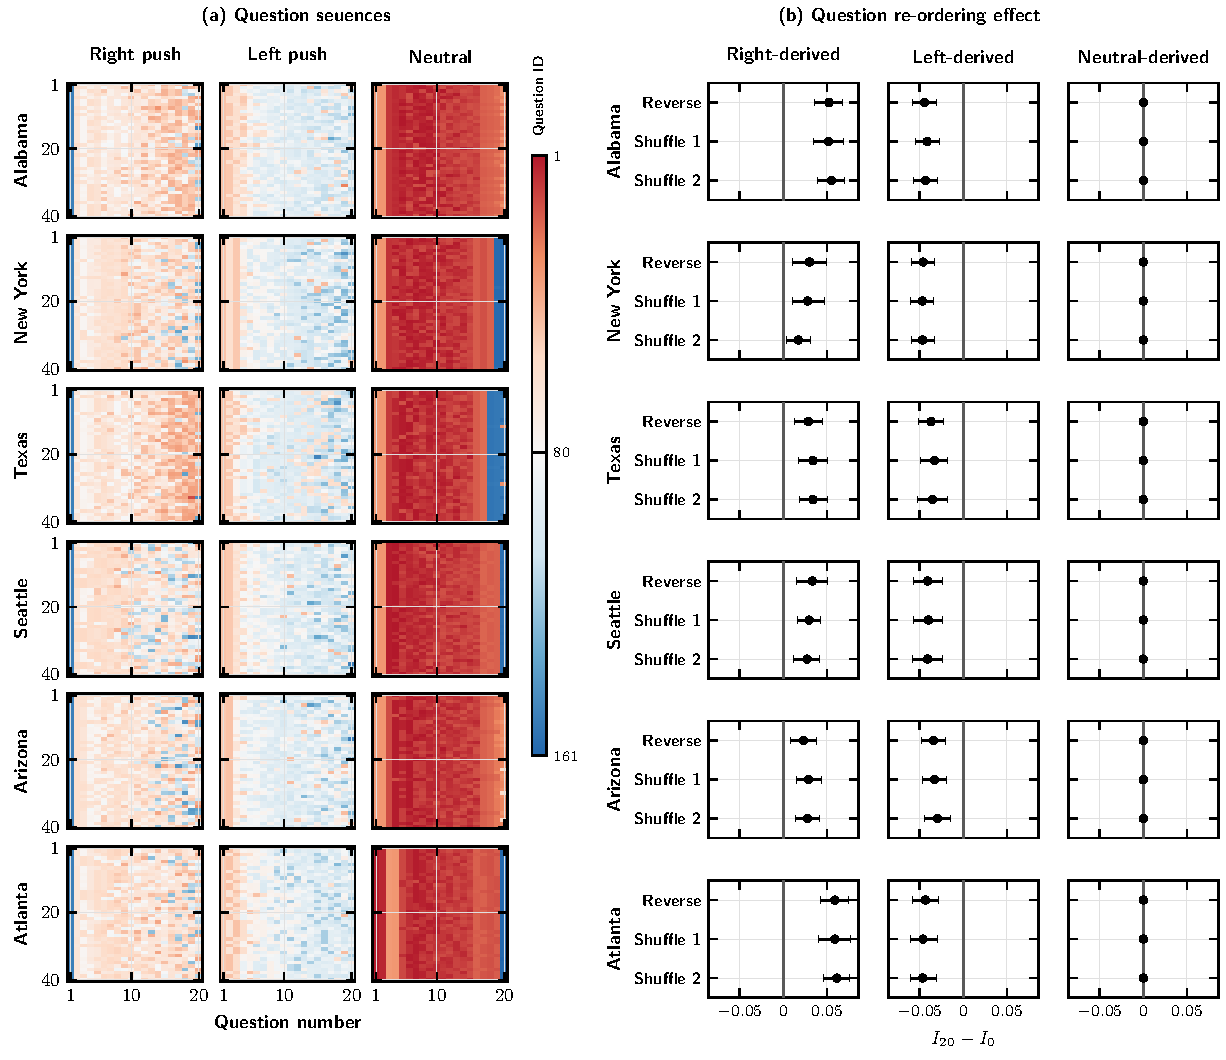
\includegraphics[width=.96\linewidth]{Figures/External/dtag-fig2.pdf}%
}{\fbox{\parbox{.89\linewidth}{Insert the already-committed fixed-set replay and question-map figure (\texttt{Figures/External/dtag-fig2.pdf}).}}}
\caption{\textbf{Extended Data Fig. 1 | Question selection and fixed-set order replays.}
The existing native panel shows selected question identities for six personas and their responses under three directional/neutral policies, and mean endpoint displacement after original, reversed and shuffled fixed-question sequences. These replays use newly sampled LSM answers rather than participant responses.}
\label{fig:nhb-order}
\end{figure}

\begin{figure}[!ht]
\centering
\IfFileExists{Figures/External/dtag-fig4.pdf}{%
  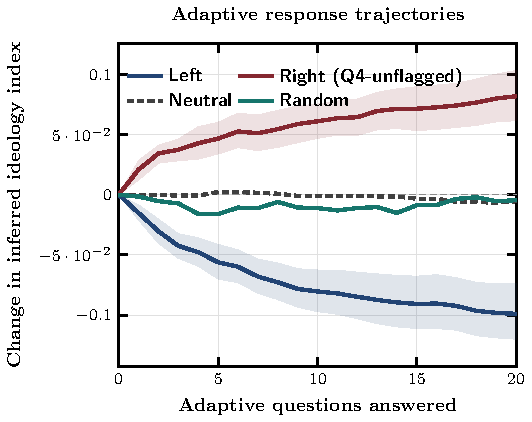
\includegraphics[width=.56\linewidth]{Figures/External/dtag-fig4.pdf}%
}{\fbox{\parbox{.53\linewidth}{Insert the Q4-filtered PGFPlots trajectory (\texttt{Figures/External/dtag-fig4.pdf}); regenerate its CSV from the private analysis export if necessary.}}}
\caption{\textbf{Extended Data Fig. 2 | Human trajectories after early Right-push resistance exclusion.}
As in the original human panel, Left ($n=21$), Neutral ($n=7$) and Random ($n=5$) display all participants. Right retains 19 of 38 participants: nine initially Right-leaning participants and ten initially Left-leaning participants not flagged by the four-question nonmovement rule. The other 19 Right-push participants are omitted from this \emph{descriptive, Q4-conditioned} series. Blue and red shading show participant-bootstrap pointwise 95\% intervals. The original, unfiltered Right-push result remains the principal comparison in Fig.~\ref{fig:nhb-human}.}
\label{fig:nhb-unflagged}
\end{figure}

\bibliographystyle{unsrtnat}
\bibliography{references,references_nhb}
\end{document}
